\chapter{Monte Carlo sull'insieme incerto lineare}
\section{Obiettivo della campagna}
M16 aggiunge una valutazione empirica sui controllori finali senza sostituire l'analisi formale M14. Il suo scopo è osservare, su realizzazioni fisiche comuni, stabilità, tracking, interazione e comando. La campagna può rivelare esempi critici e mostrare la distribuzione delle metriche nel campione; non può dimostrare proprietà per tutti i valori continui dell'insieme M4.

L'incertezza è trattata come insieme di variazioni ammissibili, non come distribuzione fisica identificata. L'estrazione uniforme implicita nel campionamento software è una regola computazionale per esplorare il dominio; le frequenze ottenute non sono quindi stime della probabilità reale di guasto del manipolatore.

\section{Disegno sperimentale e riproducibilità}
La campagna usa seed \MonteCarloSeed, generatore \texttt{twister} e \MonteCarloSamples\ campioni. La sequenza è generata una sola volta dalla pianta incerta M4. Ogni Sample ID rappresenta la stessa realizzazione fisica per M6, $K_{\infty}$ e $K_\mu$: parametri meccanici e blocchi dinamici degli attuatori non vengono riestratti passando da un controllore all'altro. Questo accoppiamento rende i confronti paired e impedisce che una differenza fra controllori dipenda da insiemi casuali diversi.

Il Sample 0 nominale è usato come controllo di implementazione e non entra nelle statistiche. Per ciascuno dei 40 campioni effettivi vengono verificati:
\begin{itemize}
\item appartenenza dei parametri reali ai range M4;
\item stabilità e bound unitario dei due blocchi dinamici campionati;
\item identità della pianta fisica usata dalle tre chiusure;
\item stabilità interna senza cancellazioni di modi;
\item metriche di tracking sugli scenari M5, cross-coupling e picco di comando.
\end{itemize}
Il replay con lo stesso seed riproduce i campioni entro la tolleranza numerica prevista.

\section{Stabilità empirica}
M6 è stabile in \MControllerStableSamples/\MonteCarloSamples\ realizzazioni. I Sample ID instabili sono \MControllerUnstableSampleIds; il peggiore presenta massima parte reale $+\MControllerWorstUnstablePole$ s$^{-1}$. Ogni caso critico viene conservato nel dataset e nella tabella: non è scartato come outlier se appartiene all'insieme di campionamento valido.

$K_{\infty}$ e $K_\mu$ sono stabili in \KhinfStableSamples/\MonteCarloSamples\ e \KmuStableSamples/\MonteCarloSamples\ campioni. La tabella distingue volutamente il numero di casi instabili dai relativi identificativi.

\begin{figure}[htbp]
\centering
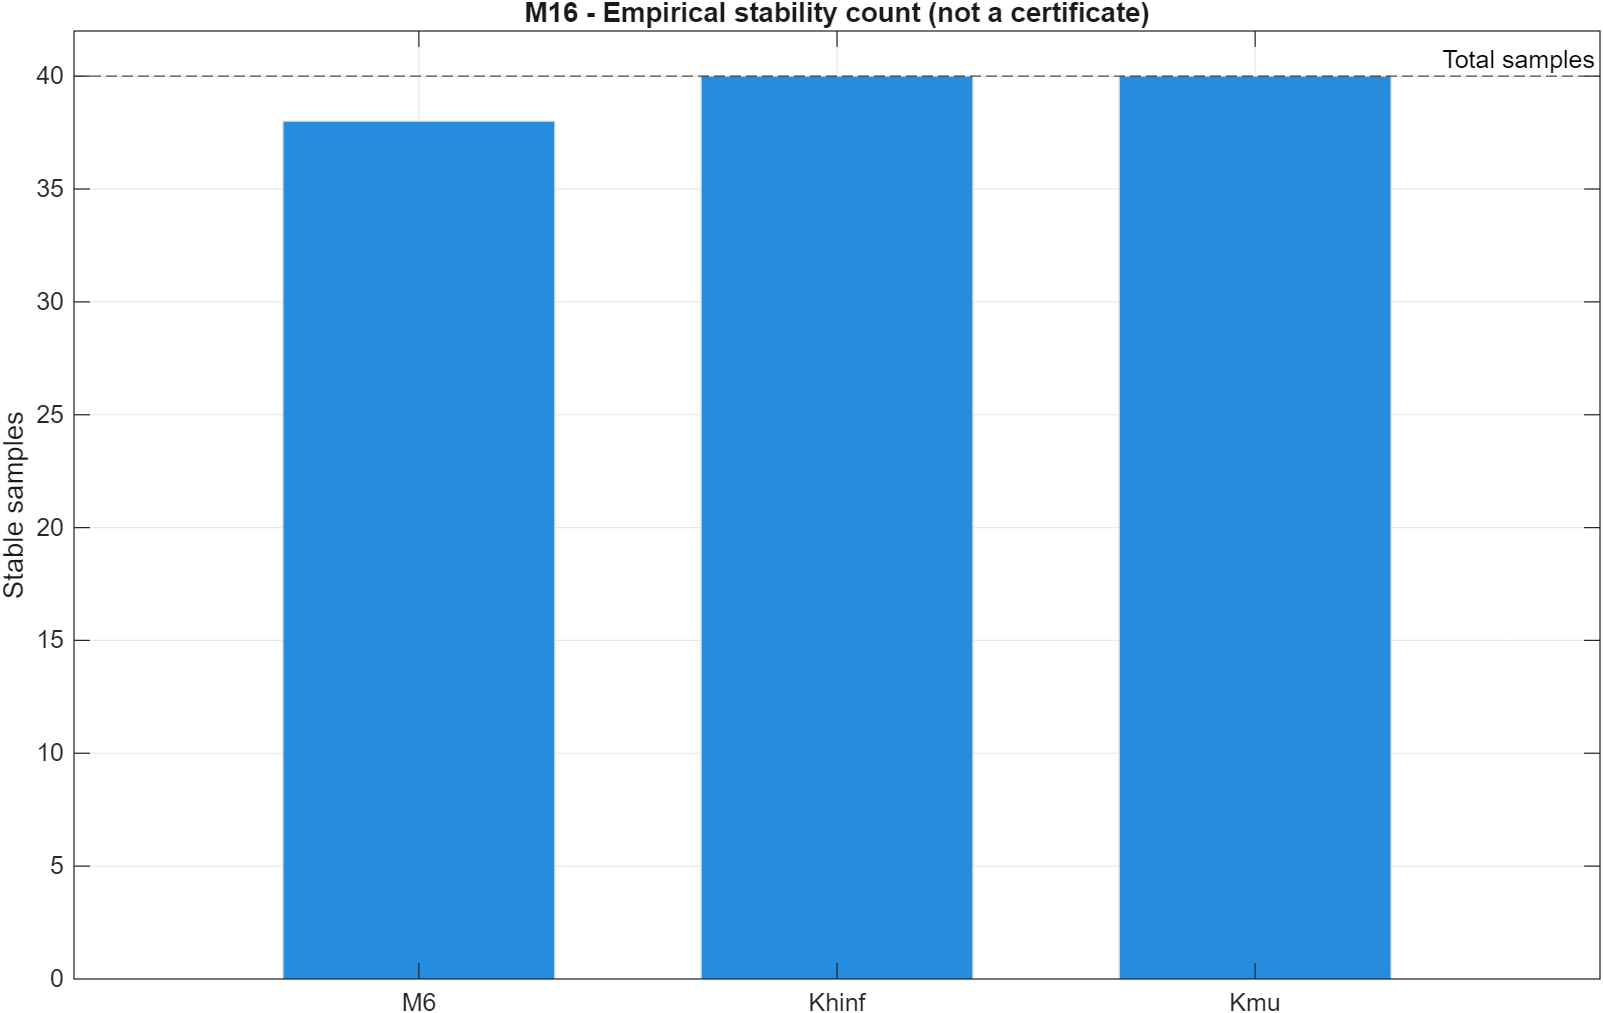
\includegraphics[width=0.62\textwidth]{figures/m16_empirical_stability_summary.png}
\caption{Stabilità osservata sui 40 campioni lineari M4. Il risultato descrive il campione finito e non l'intero insieme incerto.}
\label{fig:m16-stability}
\end{figure}

% Generated by build_m18_report_tables.m. Do not edit.
\begin{table}[H]
\centering
\resizebox{\textwidth}{!}{%
\begin{tabular}{llllll}
\toprule
Controller & Stabili & Rate [\%] & Campioni instabili & Core tracking [\%] & Peak $u$ mediano [N m] \\
\midrule
M6 & 39/40 & 97.5 & 5 & 30 & 4.6897 \\
Khinf & 40/40 & 100 & NONE & 0 & 5.1599 \\
Kmu & 40/40 & 100 & NONE & 0 & 5.1615 \\
\bottomrule
\end{tabular}
}
\caption{Monte Carlo M16: evidenza empirica lineare, non certificazione di robustezza.}
\label{tab:monte-carlo}
\end{table}


La colonna percentuale è indicata come \emph{frazione empirica} ed è calcolata dai conteggi riportati in tabella. Non è denominata probabilità di stabilità, perché mancano una distribuzione delle incertezze identificata e un'argomentazione statistica che leghi il campione alla popolazione fisica.

\section{Prestazione sui campioni stabili}
La stabilità non coincide con il rispetto del tracking. Il core tracking pass rate calcolato sul totale dei 40 campioni è \MControllerTrackingPassPct$\%$ per M6, \KhinfTrackingPassPct$\%$ per $K_{\infty}$ e \KmuTrackingPassPct$\%$ per $K_\mu$. Le frazioni osservate descrivono soltanto i campioni e i target verificati.
I casi instabili restano nel denominatore e sono esclusi dalle metriche
temporali ammissibili, senza essere occultati.

Il picco di comando è riportato come distribuzione e mediana, sempre senza confronto con una saturazione hardware. Cross-coupling e risposta al disturbo sono quantificati con le convenzioni già adottate, senza aggiungere nuove soglie dopo aver osservato i dati. L'uso degli stessi Sample ID permette di interpretare le differenze caso per caso e non mediante uno score globale.

\section{Relazione con la certificazione M14}
La nuova M14 fallisce RS: non esiste quindi una garanzia che ogni
campione M4 sia stabile. Una frazione finita di campioni stabili,
anche se fosse pari al totale, non contraddirebbe tale esito.
Il controllo di coerenza bloccherebbe invece un campione instabile
qualora esistesse una RS certificata sul medesimo insieme.
M16 non sostituisce M14 e non misura la probabilità di guasto reale.

La conclusione M16 rimane dunque empirica: nel campione comune considerato M6 è stabile \MControllerStableSamples\ volte, $K_{\infty}$ \KhinfStableSamples\ e $K_\mu$ \KmuStableSamples. La sola certificazione ammissibile richiederebbe una $\mu$-analysis indipendente positiva; M14 corrente restituisce invece RS e RP fallite.
